\chapter{Introduction}

\section{Description}

This software guide is designed to explain the concept of the firmware running on the UWB tag and all the UWB anchor devices. 
The goal is to give a understanding what classes and files are used and how the interoperate together. 
Additionally to this guide a fill Doxygen documentation will be provided. 

\section{Naming Conventions}
Within this Software Guide detailing the Time-of-Flight (TOF) function, it's important to note that the terms "initiator" and "tag" are used interchangeably. 
Both refer to the UWB (Ultra-Wideband) device responsible for initiating the TOF measurement by transmitting a UWB request to the relevant devices in its vicinity.

These devices can also be alternatively referred to as "anchor", "responder" or "landmark". This nomenclature is employed because these devices play the pivotal role of responding to the UWB request and guiding the initiator in computing the distance between them. The interchangeable use of these terms is intended to provide clarity and flexibility in describing the dynamic roles these devices undertake in the TOF measurement process.

\section{Basic functionality and setup}
The primary function of this setup revolves around the estimation of tag positions within a predefined coordinate space. 
This estimation is achieved by leveraging the distances between the tag and various anchors strategically placed within the room. 
To facilitate a clearer grasp of the setup's workings, an illustrative sketch featuring example coordinates can be found in Figure \ref{fig:setup_sketch}.
\vspace{4pt}
\newline
In this setup, the anchors are situated throughout the room in a deliberate yet arbitrary manner, each possessing known coordinates. 
The key to this system's functionality lies in the tag device's ability to discern the positions of these anchors. 
With this information, the tag can deduce its own location in all the X, Y and Z directions by gauging the distances to all the anchors.
\vspace{4pt}
\newline
In Figure \ref{fig:setup_sketch}, these distances are visually represented and labeled as d\_1 to d\_5. 
The critical aspect of this process is that it enables the tag device to employ an Extended Kalman Filter (EKF) for the purpose of position estimation. 
This filter algorithm plays a pivotal role in refining and enhancing the accuracy of the tag's estimated position within the coordinate space and is further discussed in chapter \ref{chap:EKF_Handling}. 

\begin{figure}[!hbt]
	\centering
	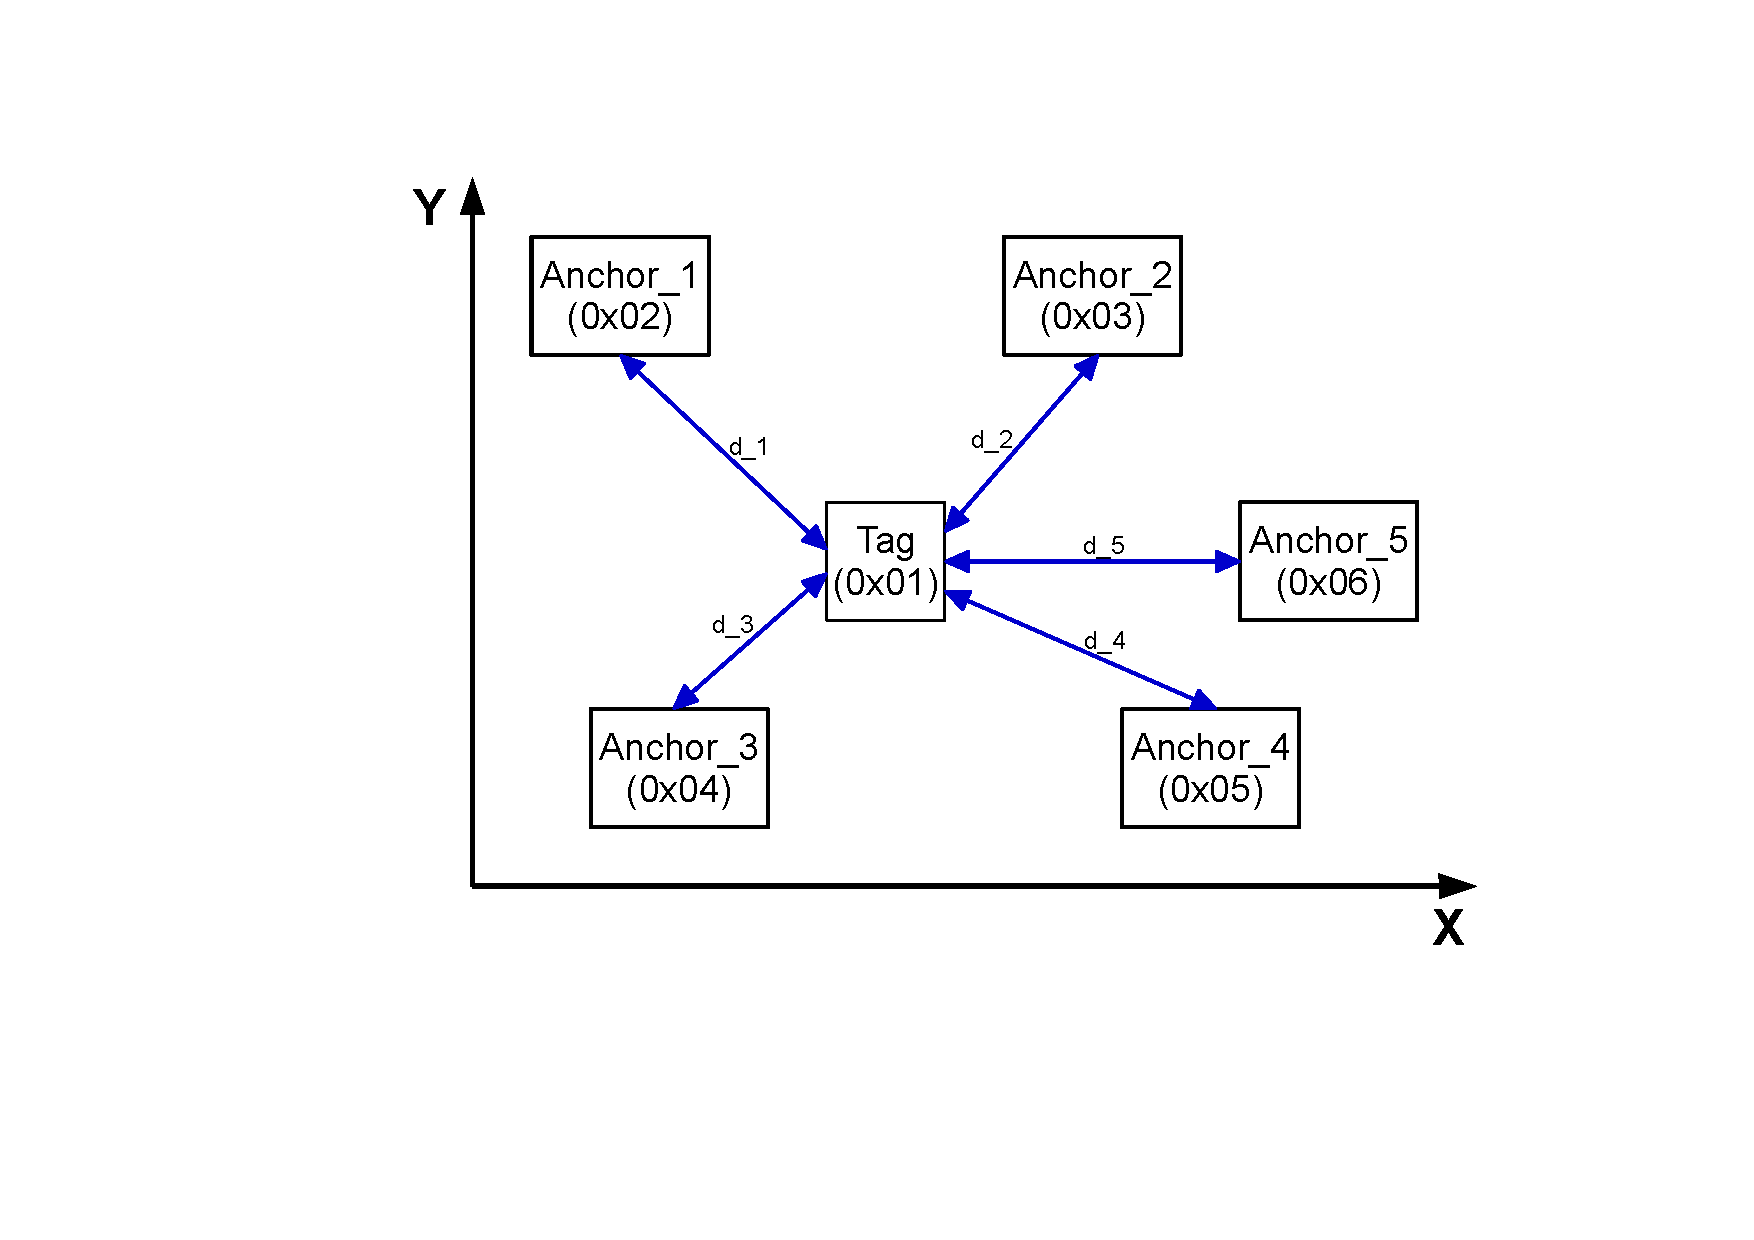
\includegraphics[width=0.6\textwidth]{pictures/Complete_Setup.pdf}
	\caption{Sketch of the complete setup.}
	\label{fig:setup_sketch}
\end{figure}

\section{Flow of Information}

In Figure \ref{fig:information_flow} the information flow of the entire system is pictured. 
The most important component are the UWB ranging messages exchanged between the Tag and every Anchor that are ultimately used to estimate the Tag's position. 
With every sent UWB message from the Tag to an Anchor the channel parameters are extracted and transmitted via WiFi to an MQTT-Server. 
The UWB Tag itself also transmits its coordinates over MQTT to a different topic. 
The MQTT mechanics are further discussed in \ref{chap:MQTT_Handling}. 
\vspace{4pt}
\newline
The configuration of the Tag, meaning putting in the coordinate of each anchor to the EEPROM, is executed via Bluetooth by a Bluetooth-Capable device running the configuration software. 
Additionally the Tag sends its position via Bluetooth where the configuration software has the ability to display it in a 2D plot in real time. 
Bluetooth Handling techniques are further elaborated in \ref{chap:Bluetooth_Handling}. 

\begin{figure}[!hbt]
	\centering
	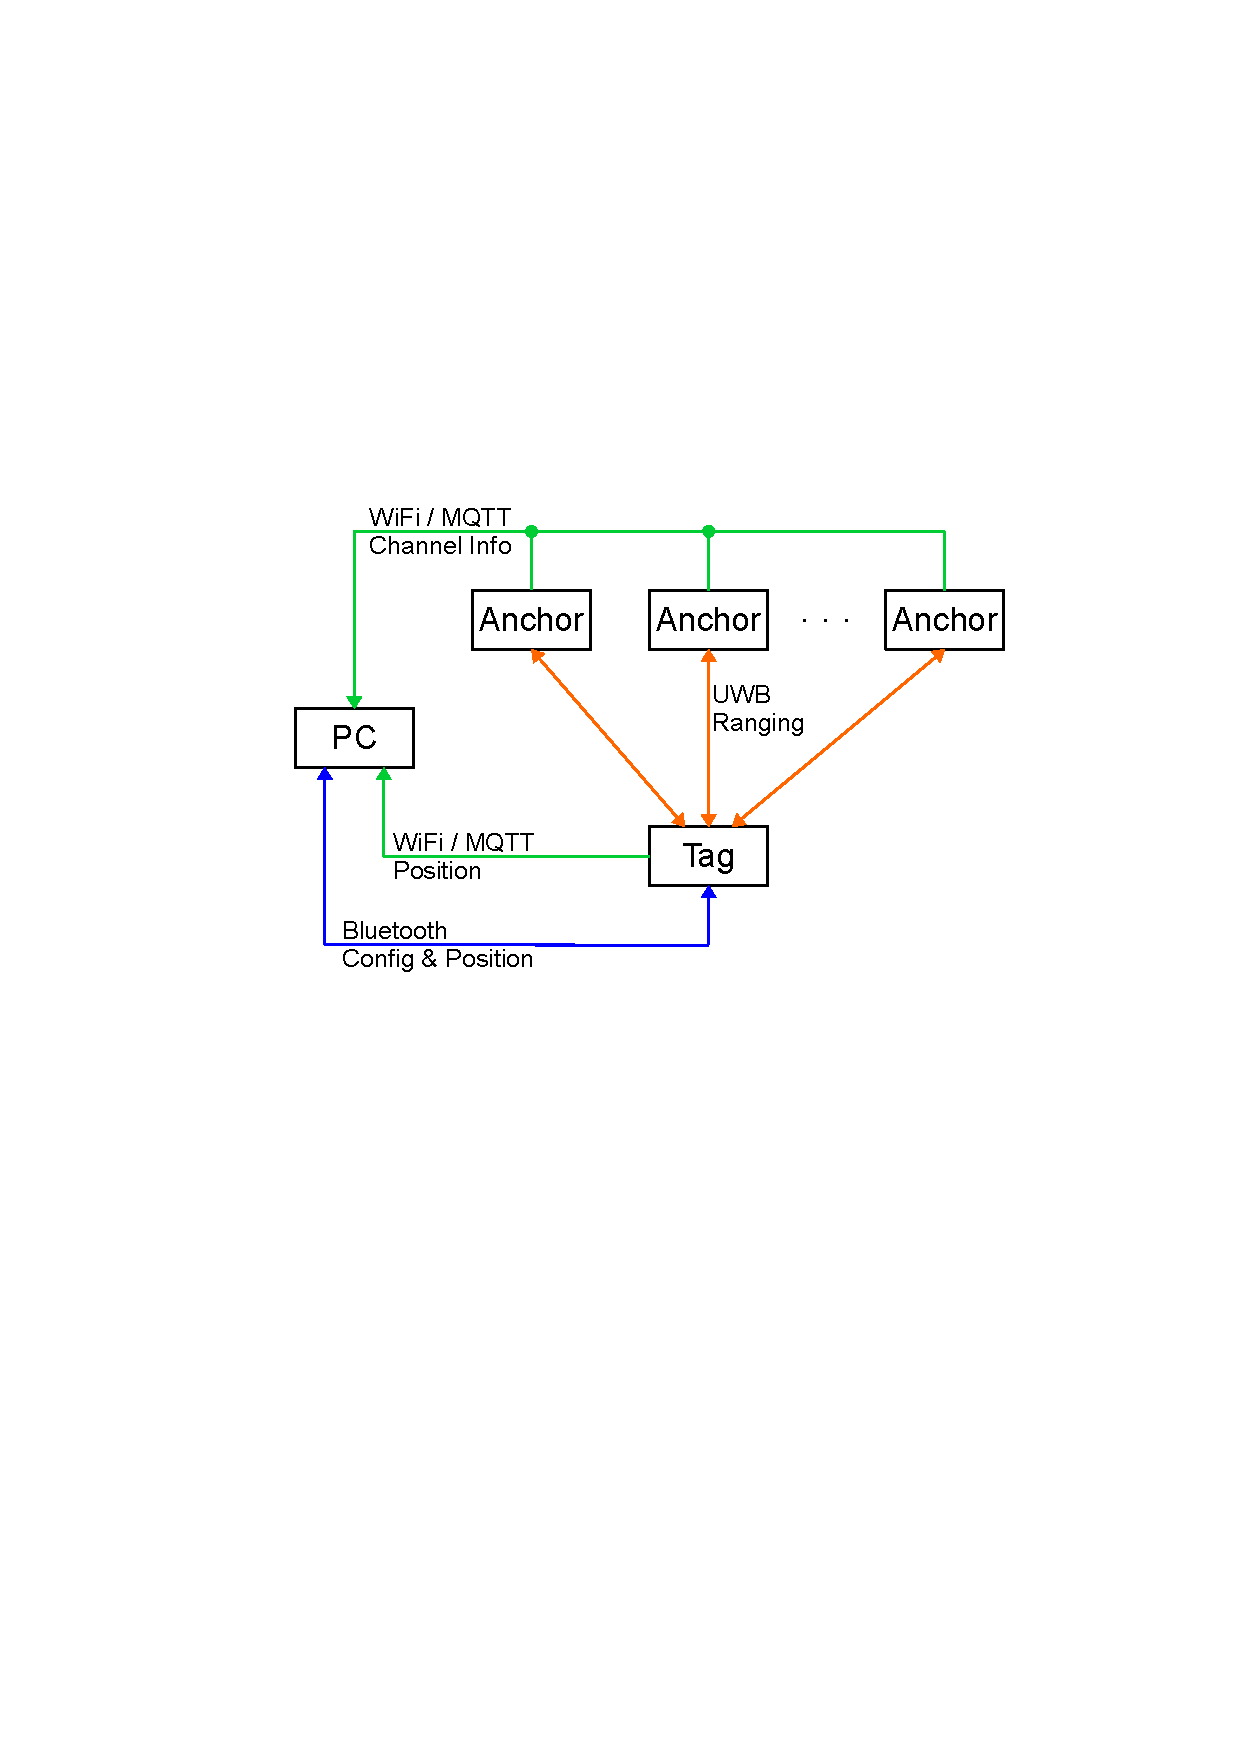
\includegraphics[width=0.6\textwidth]{pictures/information_flow.pdf}
	\caption{Sketch of the complete setup.}
	\label{fig:information_flow}
\end{figure}
